\documentclass{beamer}
\usetheme{metropolis} % Ou remplacez par votre thème préféré
\usepackage{amsmath, amsfonts, mathtools}
\usepackage{stmaryrd}
\usepackage{graphicx}
\usepackage{subcaption}
\usepackage{float}
\usepackage{tikz}
\usepackage{pgfplots}
\usepackage{bbold}
\usepackage{bm}  
\usepackage{bbm}
\usepackage{etoolbox}
\usepackage{array}
\usepackage{adjustbox}
\usepackage{caption}

\captionsetup{justification=centering}
\pgfplotsset{compat=1.18} % Version pour PGFPlots
\makeatletter
\patchcmd{\beamer@calculateheadfoot}{\insertcontinuationcount}{\relax}{}{}
\makeatother


\title{Tensor multiblock logistic regression to classify liver tumors from MRI images}
\author{SELVESTREL Alexandre}
\institute{
    Université Paris-Saclay, CNRS, CentraleSupélec, Laboratoire des signaux et systèmes\\[10 pt]
    \textbf{Supervisors :} Arthur Tenenhaus, Laurent Lebrusquet\\[10 pt]
    \textbf{Medical partner :} Henri Mondor hospital, radiologist: Sébastien Mulé
}
\date{\today}

\begin{document}

\begin{frame}
    \titlepage
\end{frame}

\begin{frame}
    \frametitle{Liver tumors classification}
    \begin{center}
        \textbf{$\mathbf{6}^{\text{th}}$ most widespread cancer and $\mathbf{4}^{\text{th}}$ mortality cause by cancer}\\
    \end{center}
    Classification:
    \begin{itemize}
        \item Hepatocellular Carcinoma (HCC): $75\%$ of cases, resection often possible\\[10 pt]
        \item CCK = Cholangiocarcinoma (CCK): $6\%$ of cases, resection difficult (possible in $30\%$ of cases)\\[10 pt]
        \item Others: benign ($18 \%$ of cases) or Hepatoblastoma ($1 \%$ of cases)
    \end{itemize}
\end{frame}

\begin{frame}
    \frametitle{Difficulties for classification}
    \begin{itemize}
    \item No perfect method using RMI images (contrast, shape, size, location): disagreement between radiologists \\[15 pt]
    \item High alpha-fetoprotein indicate HCC, but not always.\\[15 pt]
    \item Biopsy: invasive and potentially lethal ($0.02 \%$ of patients)\\
    \end{itemize}
    \begin{center}
        But a lot of clues even without biopsy $\rightarrow$ Machine Learning
    \end{center}
\end{frame}

\begin{frame}
    \frametitle{Available data}

    $\bullet$ RMI images in 3D of liver tumors (arterial, portal, late)\\[5 pt]
    $\bullet$ gender (63 men, 27 women)\\[5 pt]
    $\bullet$ age at disease (average: $63$ years old)\\[15 pt]

    From Henri Mondor hospital: Sébastien Mulé

    Same variables extracted from each RMI images 3 times (shape, texture, intensity)  $\rightarrow$ specific structure\\[10 pt]

    Need to adapt existing machine learning methods to this structure

    
\end{frame}


\begin{frame}
    \begin{figure}
        \centering
        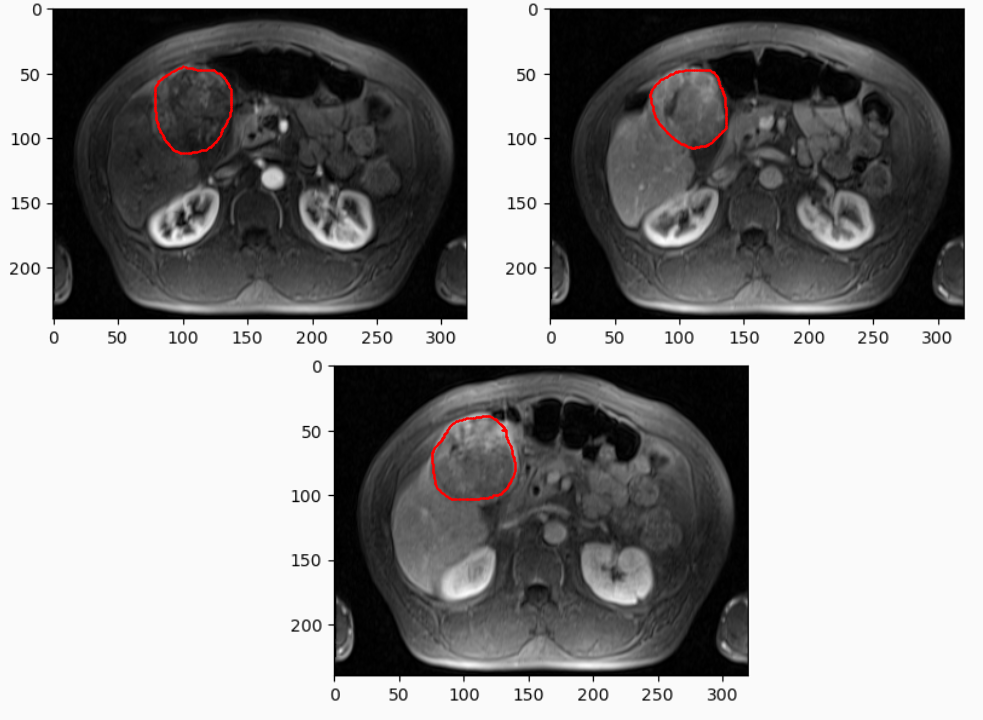
\includegraphics[scale = 0.215]{images/HCC.png}
        \caption{Example of RMI images of a HCC tumor (arterial, portal, late). More contrast in arterial}
    \end{figure}
\end{frame}

\begin{frame}
    \begin{figure}
        \centering
        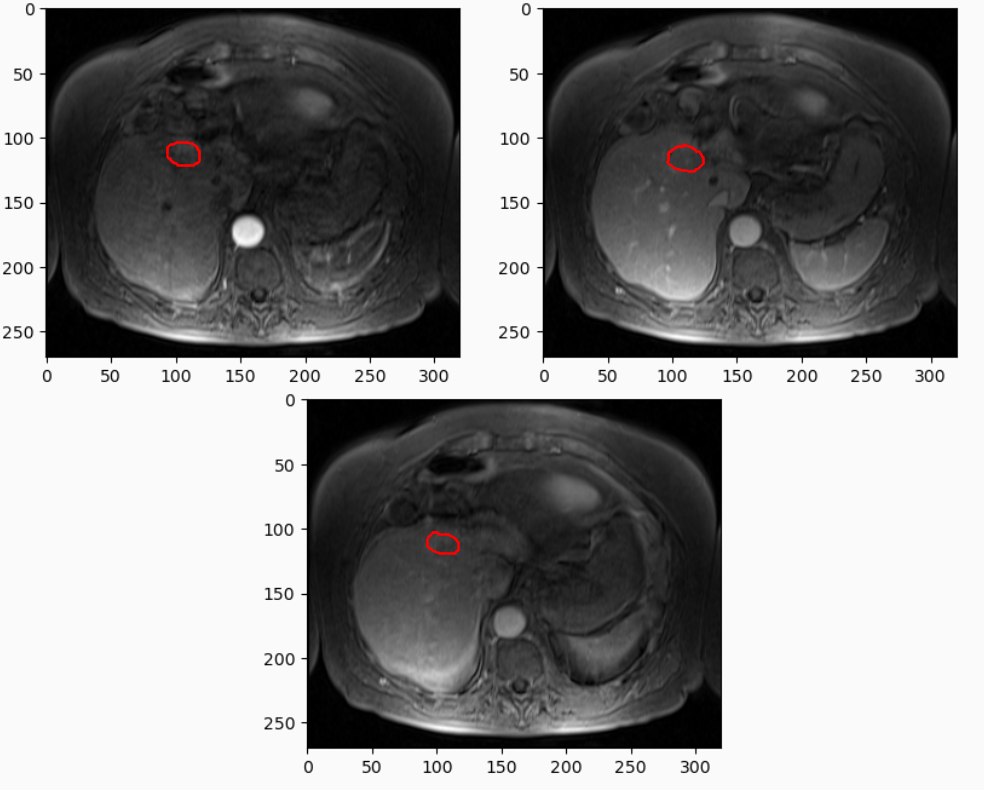
\includegraphics[scale = 0.215]{images/CCK.png}
        \caption{Example of RMI images of a CCK tumor (arterial, portal, late)}
    \end{figure}
\end{frame}


\begin{frame}
    \frametitle{Correlation matrix of the texture (GLDM) coefficients}
    Strong correlations between the imaging times for a given variable
    \begin{figure}
        \centering
        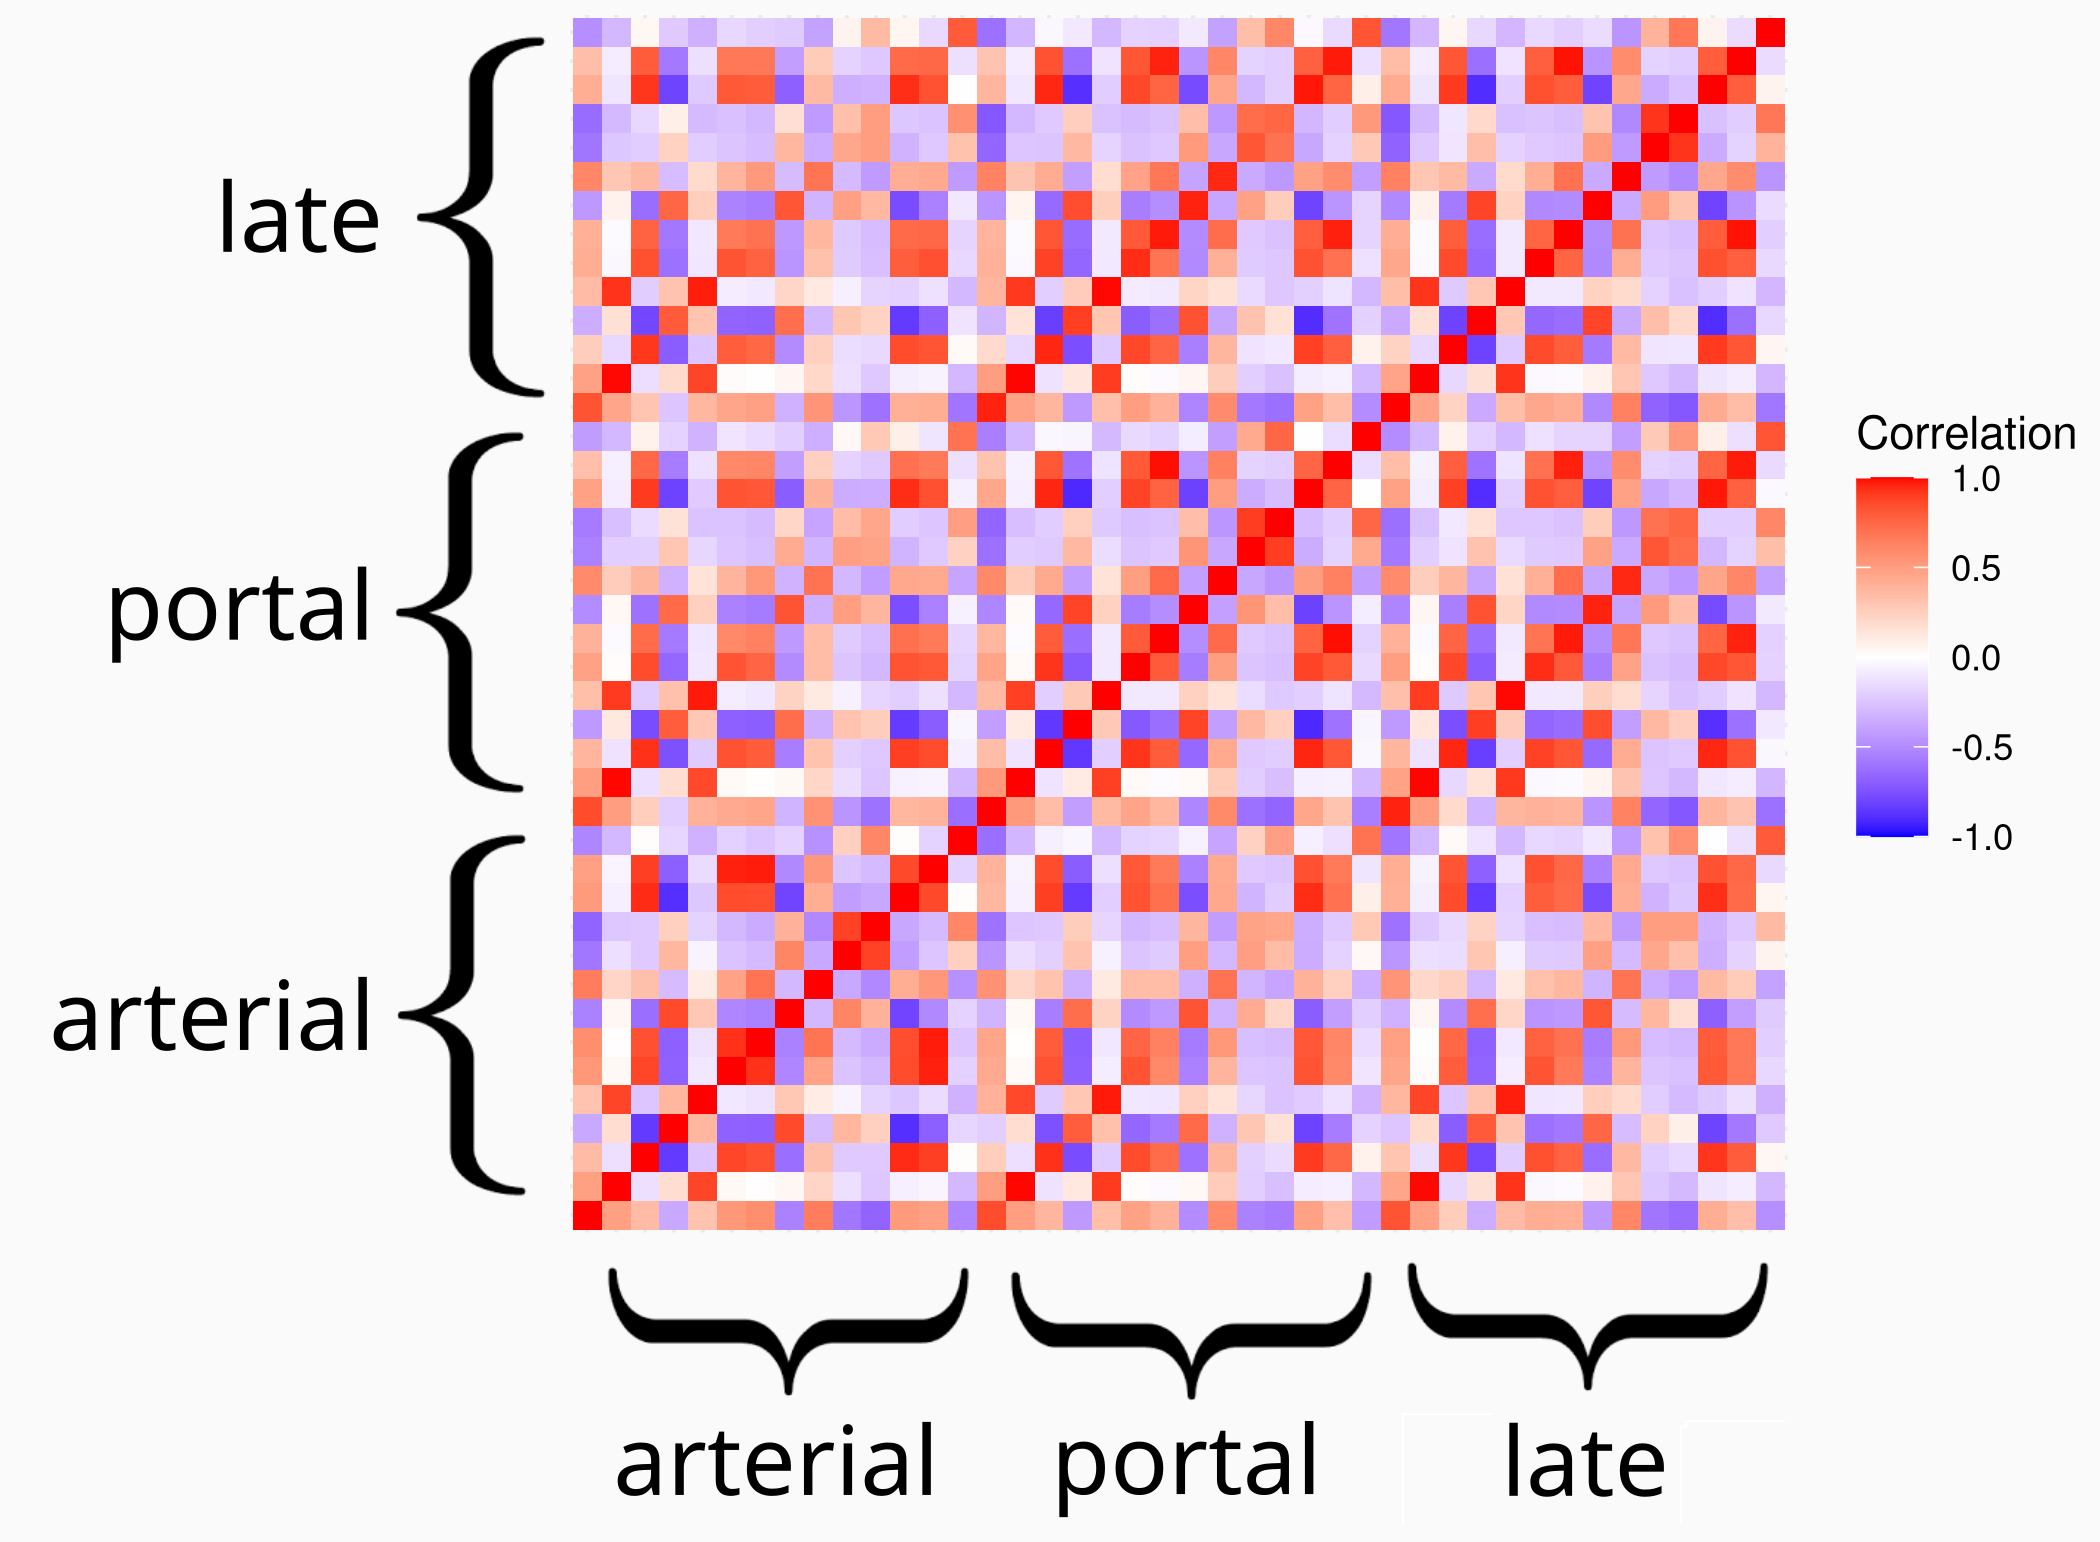
\includegraphics[scale = 0.1]{images/correlation.png}
        \caption{Correlation matrix of the texture coefficients elative to Gray Level Dependence Matrix (GLDM)}
    \end{figure}

\end{frame}

\begin{frame}
    \frametitle{Tensor data}
    Finding the best algorithm considering the structure of the data.
    \begin{figure}
        \centering
        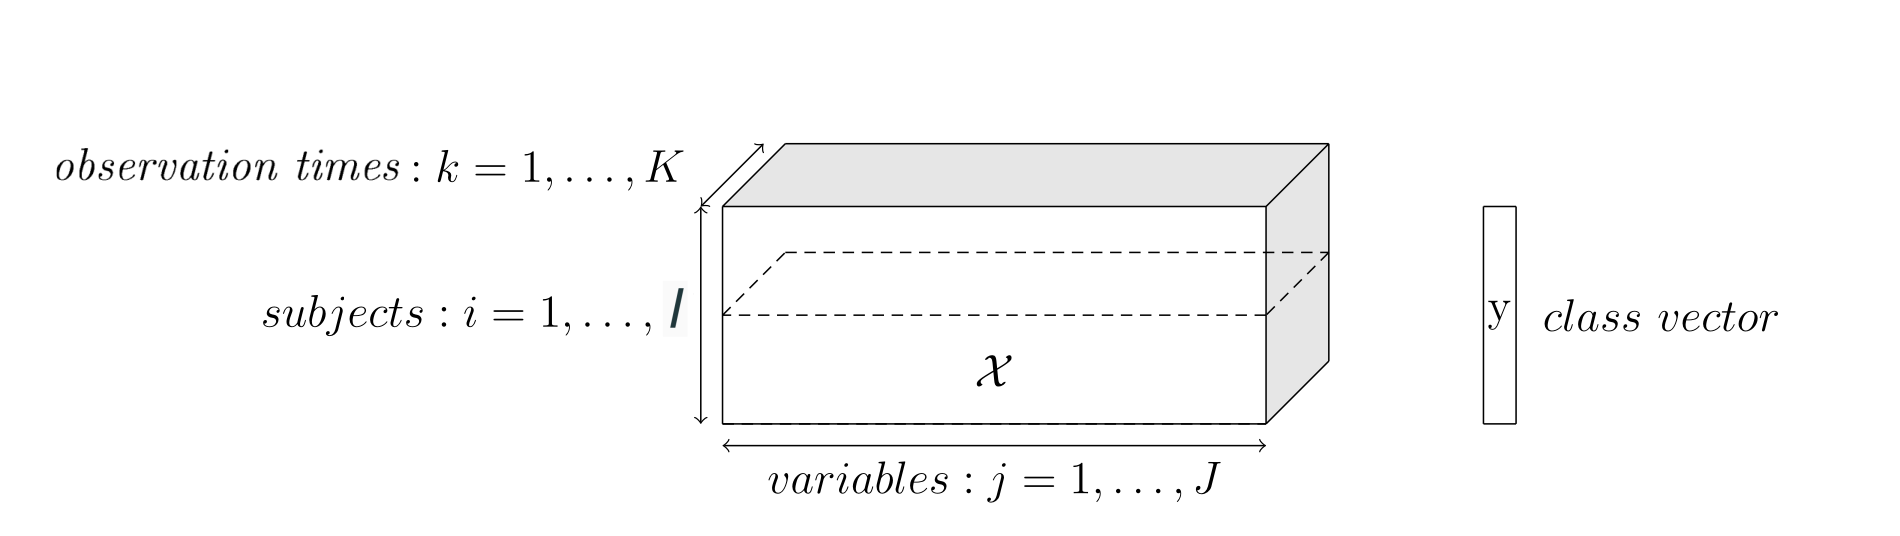
\includegraphics[scale = 0.3]{images/tensor.png}
        \caption{Type of data: tensorial}
    \end{figure}


\end{frame}

\begin{frame}
    \frametitle{Multibloc data}
    Features about pixel/voxel intensities, shape and texture: different natures
    \begin{figure}
        \centering
        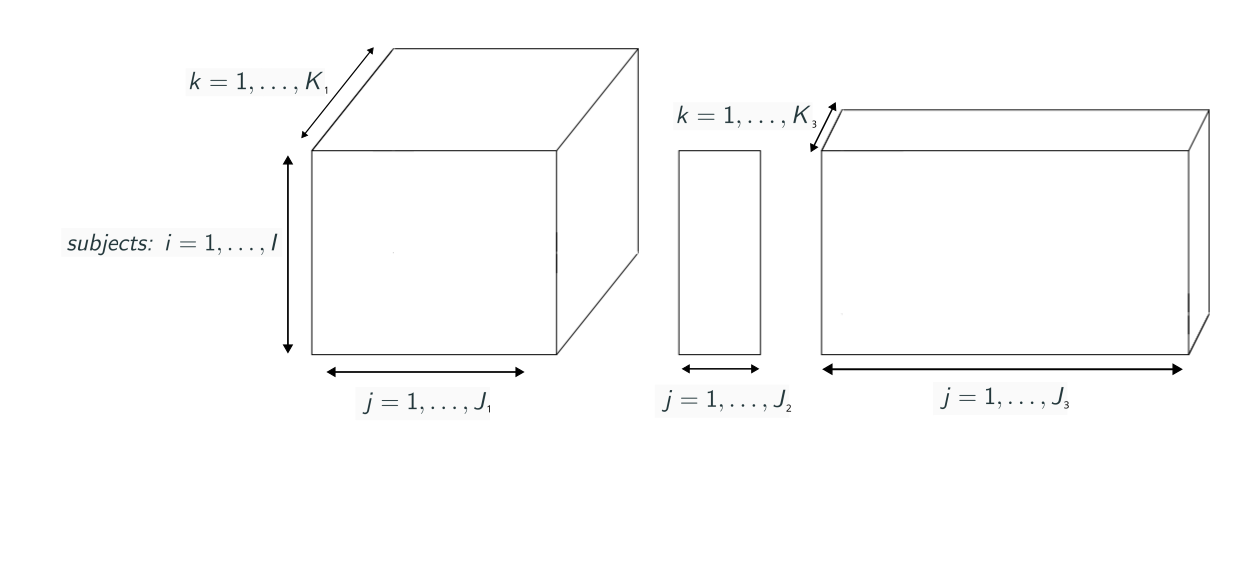
\includegraphics[scale = 0.25]{images/blocks.png}
        \caption{Type of data: multibloc}
    \end{figure}
\end{frame}



\begin{frame}
    \frametitle{Table of contents}
    \tableofcontents
\end{frame}

\begin{frame}
    \section{Machine learning models}
    \subsection{tabular models}
\end{frame}

\begin{frame}
    \frametitle{Logistic regression}
    Classical machine learning (works with few data and explainable)\\[10 pt]

    $$P(Y = 1|x) = \frac{\exp(\beta_0 + \bm{x}^T\hspace{-2 pt}\bm{\beta})}{1 + \exp(\beta_0 + \bm{x}^T\hspace{-2 pt}\bm{\beta})}$$

    Defines a likelihood function $\mathcal{L}(\bm{\beta}) = \prod_{i = 1}^I P(Y_i = y_i|x_i)$\\[15 pt]

    To much features (vs $I$) $\rightarrow$ need to limit variance of prediction. Penalization with $\lVert \bm{\beta} \rVert_1$: lasso\\[15 pt]

    function to minimize : $- \log(\mathcal{L}(\bm{\beta})) + \text{penalization}$ 
\end{frame}

\begin{frame}
    \frametitle{Impact of the tensor nature of $\bm{\beta}$}
    \begin{center}
    $\bm{\beta} = (\beta_{j,k})_{j \in \llbracket 1, J\rrbracket, k \in \llbracket 1, K\rrbracket}$ so $JK$ parameters to determine\\[15 pt]
    \end{center}
    $$x^T \bm{\beta} \leadsto \sum\limits_{k}\sum\limits_{j}  \beta_{j,k} x_{j,k} \hspace{0.5 cm} \text{and} \hspace{0.5 cm} \lVert \bm{\beta} \rVert_1 = \sum\limits_{k}\sum\limits_{j} \lvert \beta_{j,k} \rvert$$
    \begin{figure}
        \centering
        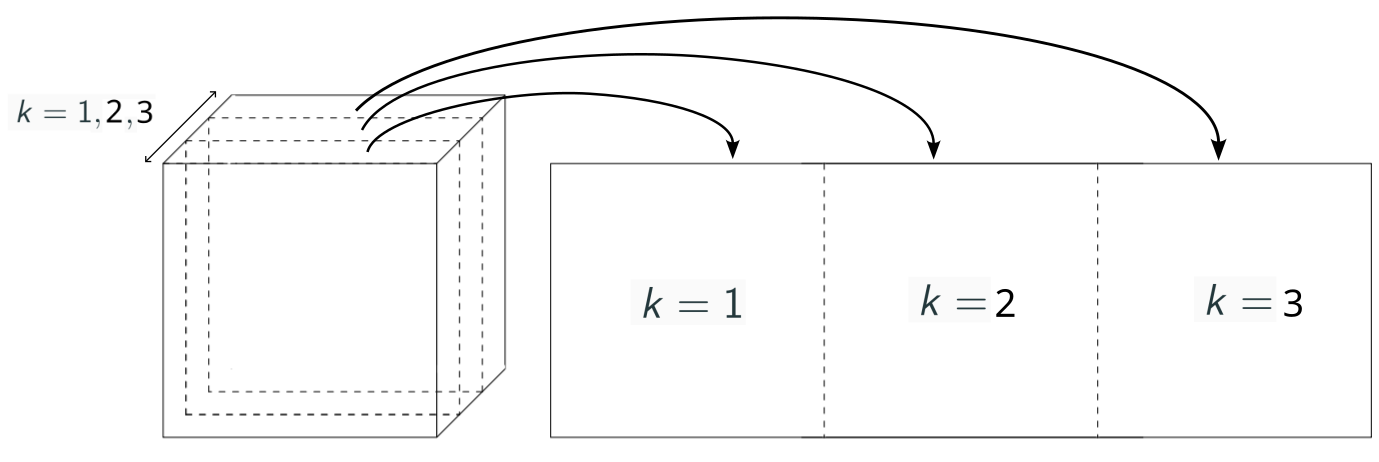
\includegraphics[scale = 0.2]{images/deplier.png}
        \caption{Unfolding of a tensor}
    \end{figure}

    
\end{frame}

\begin{frame}
    \frametitle{Group lasso}
 \textbf{Limitation of lasso}: Elimination of features without specific considerations for the same feature at other times/ other features at the same time\\[10 pt]

 Common solution: grouping coefficients together in the penalization
 $$ \sum\limits_{j,k} |\beta_{j,k}|\leadsto \sum\limits_{g = 1}^G \lVert \bm{\beta}^g \rVert_2 $$

 Tendency to cancel variables by entire blocks.

\textbf{But}: grouping either by mode or by variable, not both.  Adapting the model to the structure of the data (aim of the internship)
    

\end{frame}

\subsection{tensor models}
\begin{frame}
    \frametitle{Tensor regression models}
    Idea: each variable and mode has its own influence on the prediction (i.e. on $\bm{\beta}$) \cite{multi_rank_1}.\\[10 pt]
    \begin{overprint}
    \onslide<1>
    \begin{figure}
        \centering
        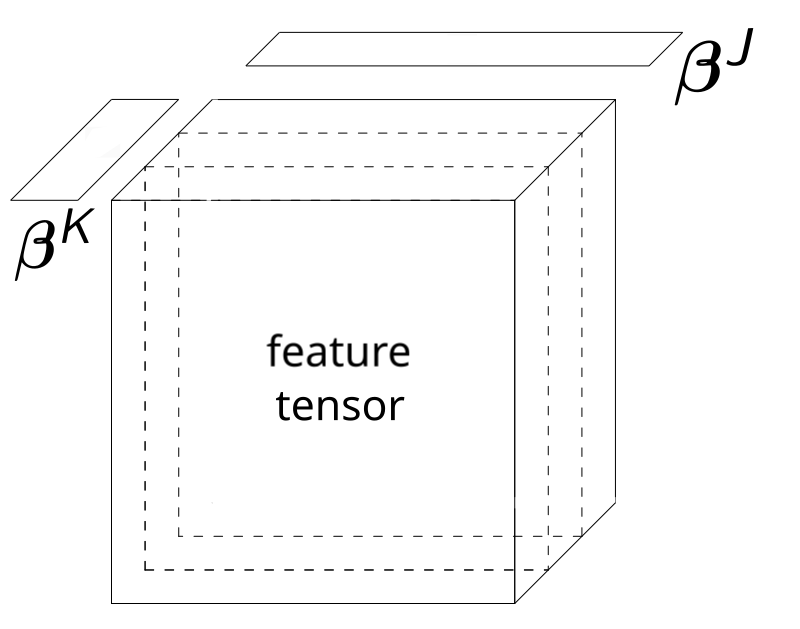
\includegraphics[scale = 0.3]{images/beta_tens.png}
        \caption{Tensor structure of $\bm{\beta}$}
    \end{figure}
    \onslide<2>
    \vspace{10 pt}
    For $J$ variables observed following $K$ modalities (e.g. times)
    $$\beta_{j,k} = \beta_j^J\beta_{k}^{K}$$
    $\beta_j$ : impact of variable $j$\\[5 pt]
    $\beta_k$ : impact of modality $k$\\[10 pt]
    Only $J+K$ parameters to determine (instead of $JK$)
    
\end{overprint}
\end{frame}

\begin{frame}
    \frametitle{Limits of rank $1$}
    \vspace{10 pt}
    \hspace{60pt} $\beta_{j,k} = \beta_j^J\beta_{k}^{K}$ implies that $\bm{\beta}$ looks like:
    \begin{figure}
        \centering
        \begin{minipage}{0.3\textwidth}
            \centering
            
\includegraphics[width=\textwidth]{images/square.png}
            \caption{\centering Example of rank 1 pictogram (only 0 and 1)}
        \end{minipage}
        \hspace{0.1\textwidth}
        \begin{minipage}{0.4\textwidth}
            \centering
            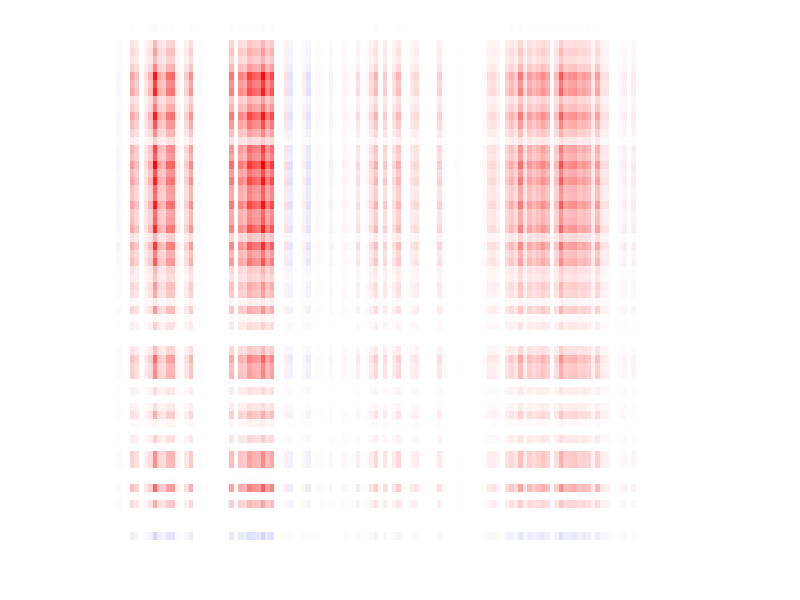
\includegraphics[width=\textwidth]{images/picto_500/heatmap_logistic_multibloc_simu_500_multiway.png}
            \caption{\centering Example of rank 1 matrix (all values allowed)}
        \end{minipage}
    \end{figure}
    \begin{center}
        \vspace{5 pt}
        This can be too simplistic
    \end{center}


\end{frame}

\begin{frame}
    \frametitle{Rank R tensor logistic regression \cite{multi_rank_r}}
    \hspace{50 pt}Summing rank 1 together : $\beta_{j,k} = \sum\limits_{r = 1}^R \beta_{j,r}^J\beta_{k,r}^K$\\
    % $$\beta_{j,k}x_{j,k} = \left( \sum\limits_{r = 1}^R \beta_{j,r}^J\beta_{k,r}^K \right) x_{j,k} = \sum\limits_{r = 1}^R \beta_{j,r}^J\beta_{k,r}^K \hspace{1 pt} x_{j,k}$$
    \vspace{-10 pt}
\begin{figure}
    \centering
    \begin{minipage}{0.5\textwidth}
        \centering
        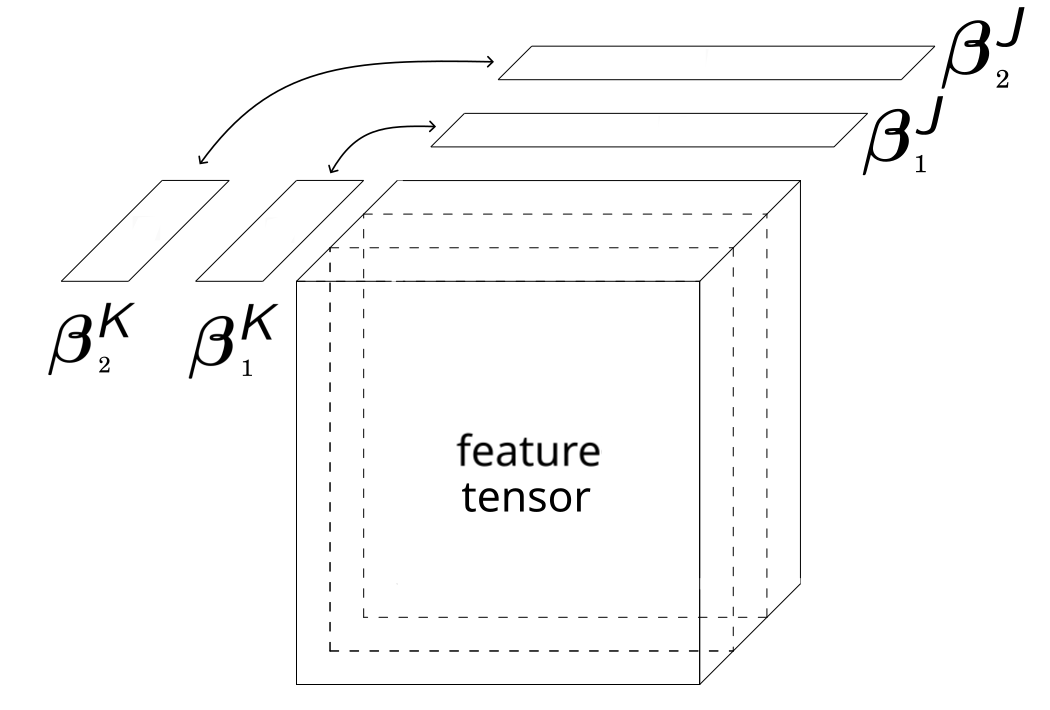
\includegraphics[scale=0.25]{images/beta_tens_R.png}
        \caption{Tensor structure of $\bm{\beta}$}
    \end{minipage}
    \hfill
    \begin{minipage}{0.45\textwidth}
        \centering
        % Ajoutez votre équation ici
        \[
        \text{lasso} \leadsto  \sum\limits_{r = 1}^R \left( \lVert \bm{\beta}_{(1,r)}^J \rVert_1 \lVert \bm{\beta}_{(1,r)}^K \rVert_1 \right)
        \]
    \end{minipage}
\end{figure}
\end{frame}

\begin{frame}
 \frametitle{Blocs of variables}

 \textbf{Problem}: Several groups of variables of different natures (first order, shape, texture). But $\bm{\beta}_r^{K}$ and $\bm{\beta}_r^J$ common to all groups.$K_1 = K_2 = K_3$ needed or else:

 \begin{figure}
    \centering
    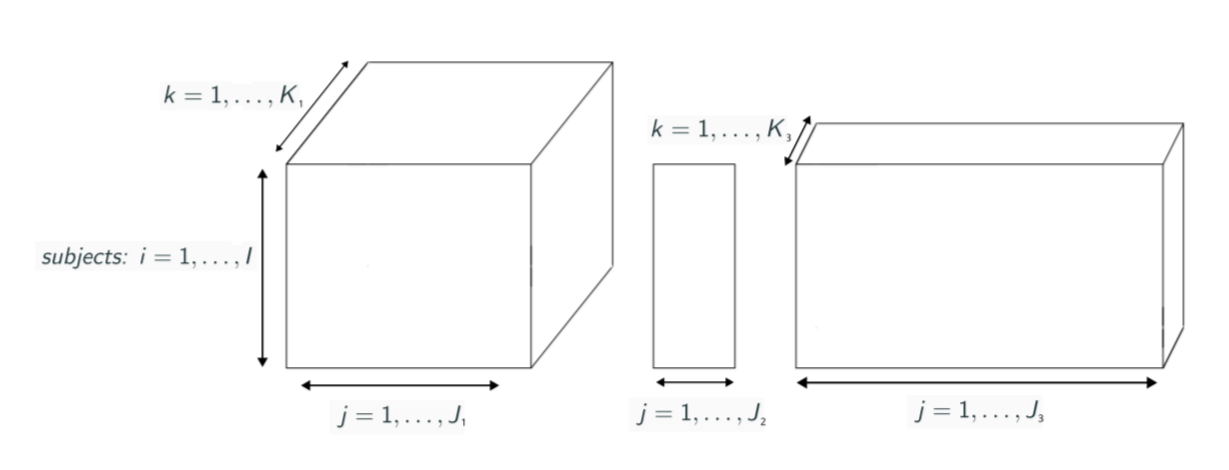
\includegraphics[scale = 0.23]{images/blocks_faux.png}
    \caption{Problem if blocs have different order or dimensions}
\end{figure}

\end{frame}

% \begin{frame}
%     \frametitle{Multiway model with blocs of variables}
%     If $K_1 = K_2$, blocks can be glued, but the structure is lost
%     \begin{figure}
%         \centering
%         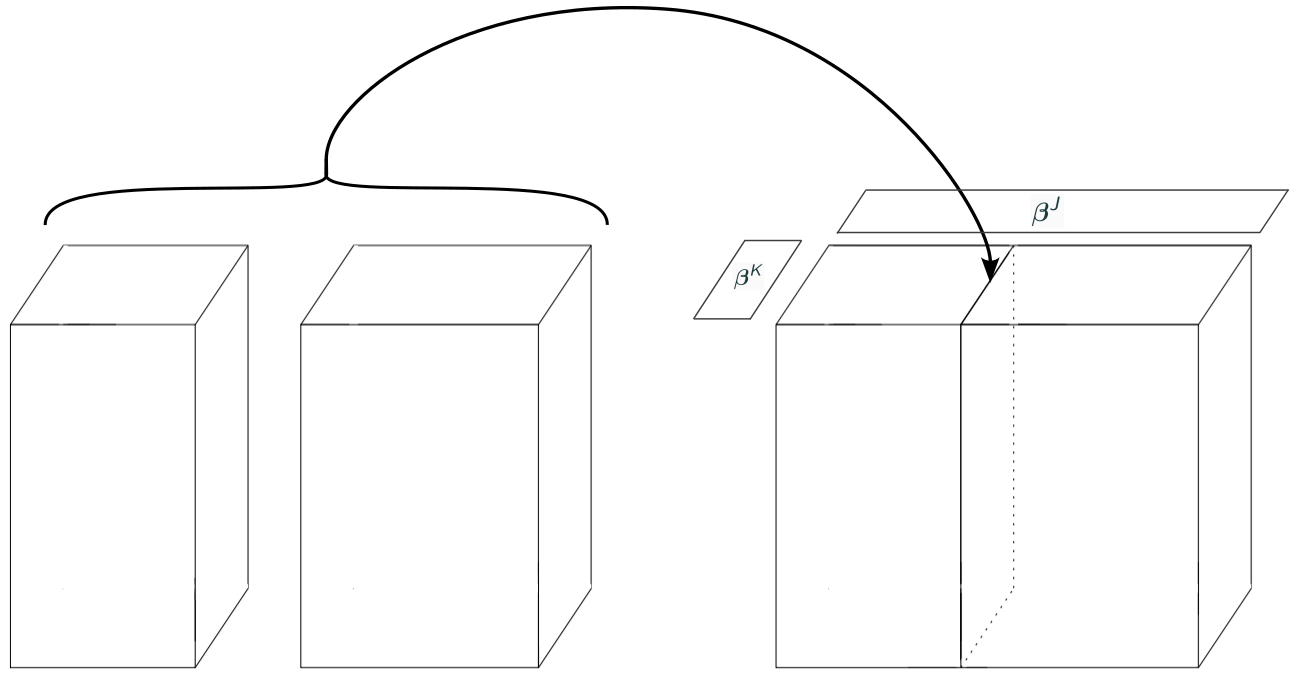
\includegraphics[scale = 0.2]{images/glue_blocks.png}
%         \caption{Multiway model with blocs of variables}
%     \end{figure}
% \end{frame}

\begin{frame}
    \frametitle{Tensor multiblock logistic regression}
    \vspace{10 pt}
    \textbf{Solution}: giving each block its own $\bm{\beta}^J$ and $\bm{\beta}^K$\\[15 pt]
    \begin{figure}
        \centering
        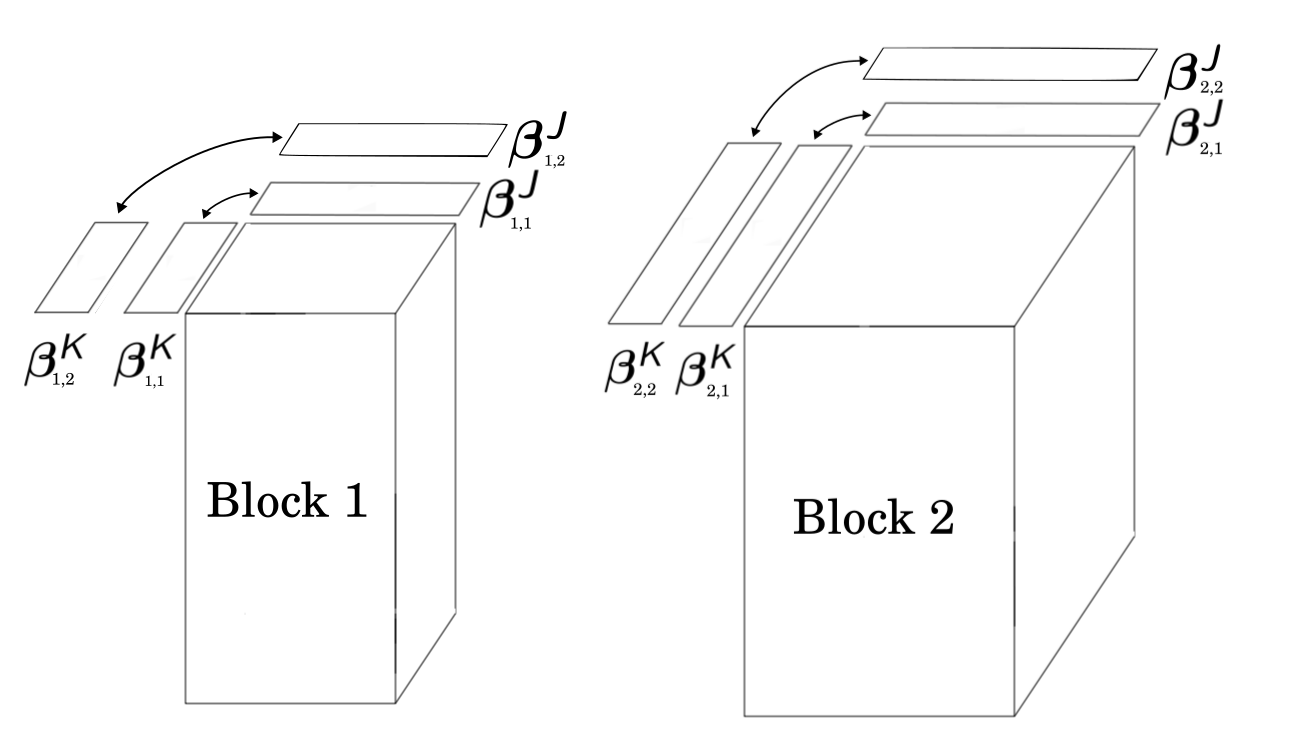
\includegraphics[scale = 0.28]{images/beta_blocks.png}
        \caption{Tensor multiblock model for rank 1}
    \end{figure}
\end{frame}

\begin{frame}
    \frametitle{Tensor multiblock logistic regression}
    Mathematically, this gives :
    $$\mathbf{x}^T\bm{\beta} \leadsto =  \sum\limits_{l = 1}^L \sum\limits_{j,k} x_{j,k}^l\beta_{j,k}^l$$
    With, for rank 1: $\beta_{j,k}^l = \beta_j^{J_l}\beta_k^{K_l}$\\[10 pt]
    But each $\bm{\beta}^l$ can have a different rank $R_l$, which gives:
    $$\beta_{j,k}^l = \sum\limits_{r = 1}^{R_l} (\beta_r^{J_l})_j \, (\beta_r^{K_l})_k $$
\end{frame}

\begin{frame}
    \section{Simulations}    
\end{frame}

\begin{frame}
    \frametitle{Parameters to control:}
    \begin{itemize}
        \item Difficulty of the classification (overlap between classes, distance between means of classes etc ...)\\[12 pt]
        \item Balance between classes\\[12 pt]
        \item Structure of the regression coefficients $\bm{\beta}$ (several blocks)\\[12 pt] 
        \item Quality of the classification (AUC)\\[12 pt]
        \item Quality of the reconstruction of $\bm{\beta}$ \nocite{picto}
    \end{itemize}
\end{frame}

\begin{frame}
    \frametitle{Illustration in 2D}

    \begin{figure}
        \centering
        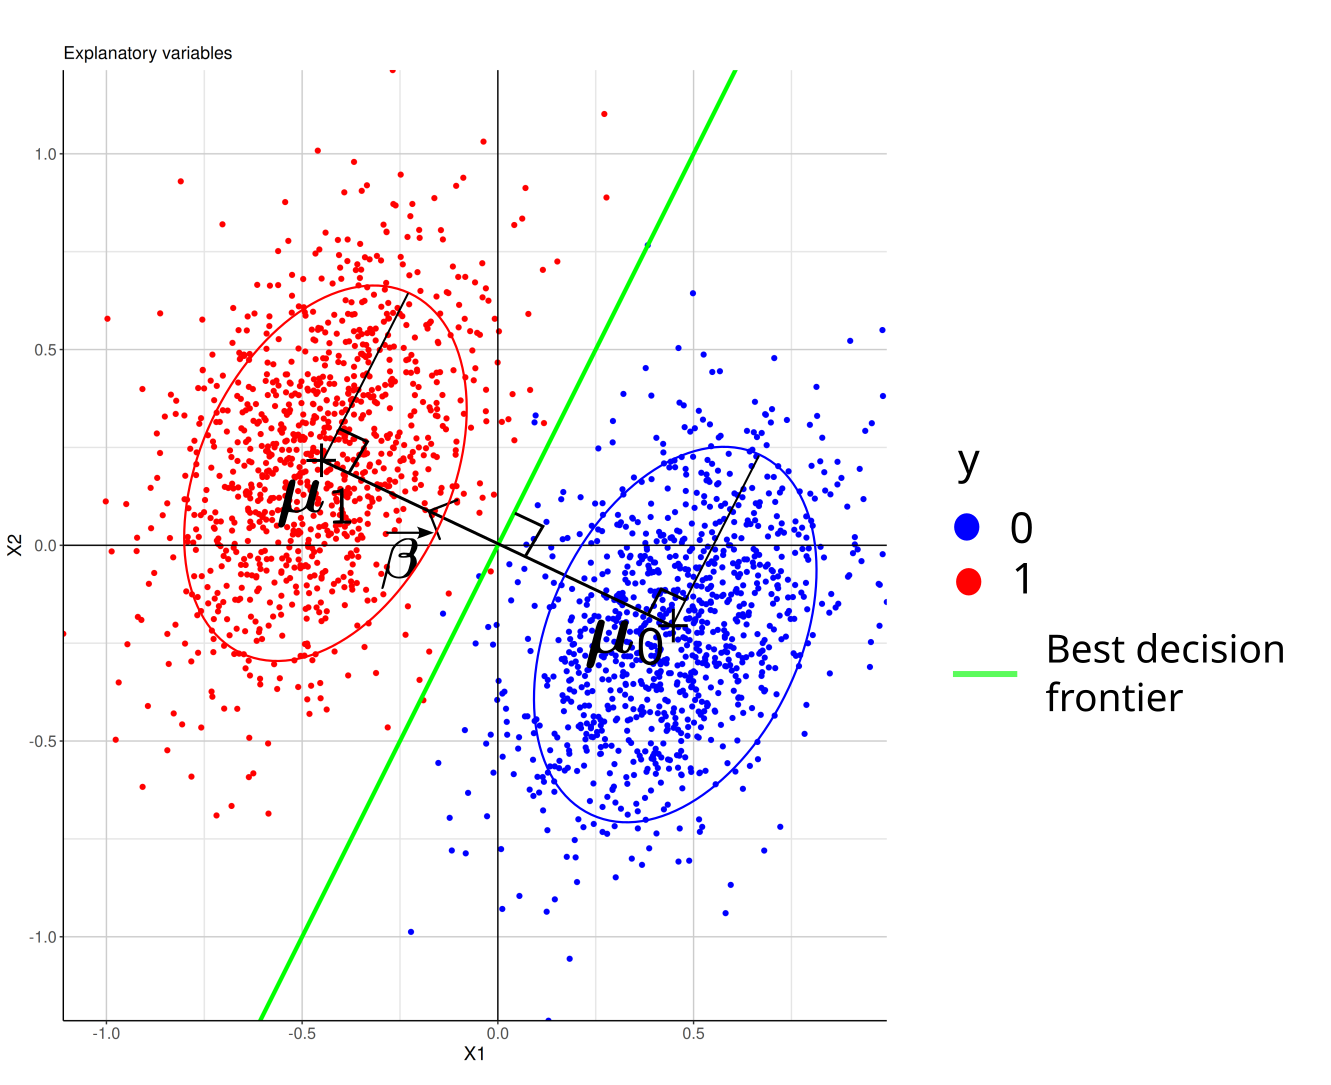
\includegraphics[scale = 0.2]{images/2D_better.png}
        \caption{Example of explanatory variables for $\bm{\beta} = (-2,1)$}
    \end{figure}
\end{frame}

\begin{frame}
    \frametitle{Data generation}
    Chose the $\bm{\beta}$ to be reconstructed (pictograms)\\[10 pt]
    Generate the $(\mathbf{x}_i)_{i \in \llbracket 1, I\rrbracket}$ with 2 multivariate normal laws of means $\bm{\mu}_0$ and $\bm{\mu}_1$ and common covariance matrix $\bm{\Sigma}$ such that:
    \begin{itemize}
        \item $\bm{\mu}_1 - \bm{\mu}_0$ colinear to $\bm{\beta}$\\[10 pt]
        \item One of the principal axis of $\bm{\Sigma}$ colinear to $\bm{\beta}$
    \end{itemize}
    Separation of classes linked with eigenvalues of $\bm{\Sigma}$ (to be compared with $\lVert\bm{\mu}_1 - \bm{\mu}_0 \rVert$)
\end{frame}

\begin{frame}
    \frametitle{AUC simulated data}
    \begin{figure}
        \begin{table}[H]
            \centering
            \caption{Cross validated AUC for each model on simulated data for 3000 individuals}
            \label{tab:result_simul}
            \renewcommand{\arraystretch}{1.2} 
            \begin{adjustbox}{center}
            \begin{tabular}{|>{\centering\arraybackslash}m{1.7cm}|>{\centering\arraybackslash}m{1.1cm}|>{\centering\arraybackslash}m{1.1cm}|>{\centering\arraybackslash}m{1.1cm}|>{\centering\arraybackslash}m{1.1cm}|>{\centering\arraybackslash}m{1.1cm}|>{\centering\arraybackslash}m{1.1cm}|}
                \cline{1-7}
                $(\sigma_{\bm{\beta}}, \sigma_{\text{noise}})$ & lasso & g.l. (blocs) & g.l. (mode)& g.l. (var) & tensor & tensor blocks\\
                \cline{1-7} 
                (0.1,0.5) & 0.83 & 0.86 & 0.94 & 0.94 & 0.99 & 0.99 \\
                \cline{1-7}
                (0.1,0.8) & 0.63 & 0.64 & 0.68 & 0.68 & 0.93 & 0.99 \\
                \cline{1-7}
            \end{tabular}
        \end{adjustbox}
        \end{table}
    \end{figure}
    
    \begin{figure}
        \centering
        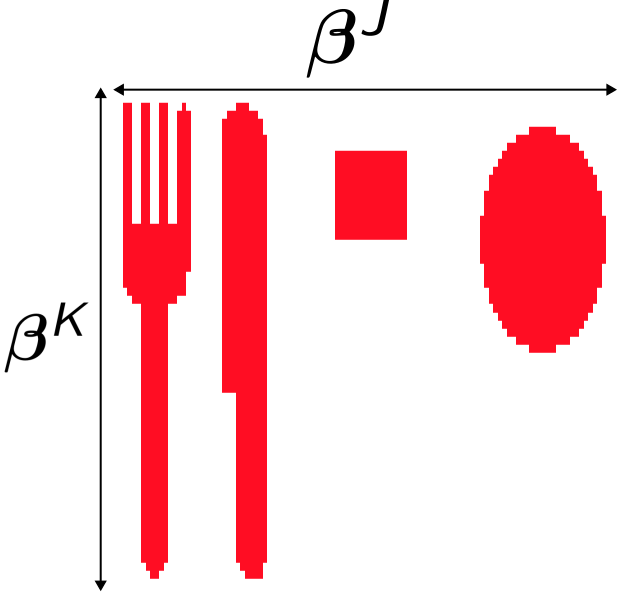
\includegraphics[scale = 0.12]{images/3_picto.png}
        \caption{Pictogram of shape $66 \times 117$}
    \end{figure}

\end{frame}

\begin{frame}

    \frametitle{Reconstructed $\bm{\beta}$}
    \begin{figure}[H]
        \centering
        \begin{minipage}{0.30\textwidth}
            \centering
            \subfloat[lasso $(\sigma_{\bm{\beta}}, \sigma_{\text{noise}}) = (0.1,0.5) $\label{fig:3000simple}]{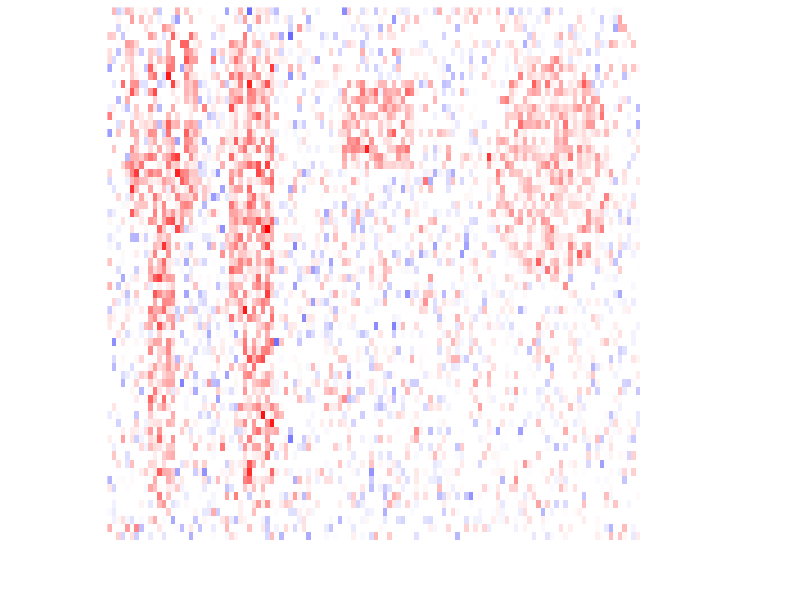
\includegraphics[width=\textwidth]{images/heatmap_logistique_simple_simu_4000.png}}
        \end{minipage}
        \begin{minipage}{0.30\textwidth}
            \centering
            \subfloat[tensor $R: 10$ $(\sigma_{\bm{\beta}}, \sigma_{\text{noise}}) = (0.1,0.5) $\label{fig:3000simple}]{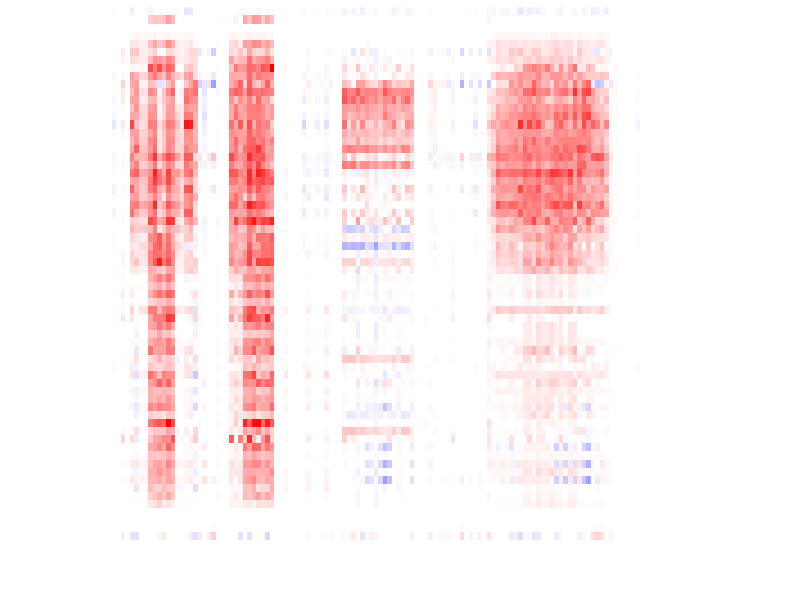
\includegraphics[width=\textwidth]{images/heatmap_logistic_multibloc_simu_4000_multiway.png}}
        \end{minipage}
        \begin{minipage}{0.30\textwidth}
            \centering
            \subfloat[T.M. $R: (12,1,10)$ $(\sigma_{\bm{\beta}}, \sigma_{\text{noise}}) = (0.1,0.5) $\label{fig:multiblock}]{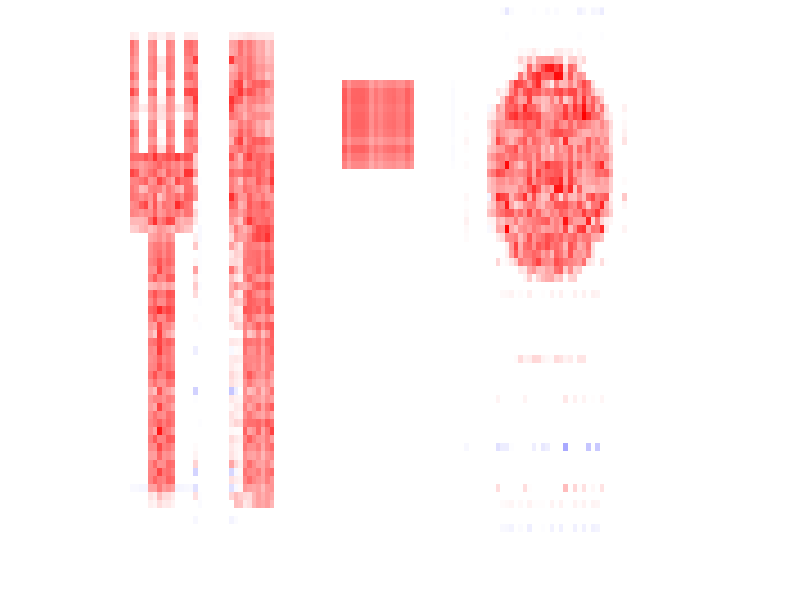
\includegraphics[width=\textwidth]{images/heatmap_logistic_multibloc_simu_4000.png}}
        \end{minipage}
        \begin{minipage}{0.30\textwidth}
            \centering
            \subfloat[lasso $(\sigma_{\bm{\beta}}, \sigma_{\text{noise}}) = (0.1,0.8) $\label{fig:easy_multiblock}]{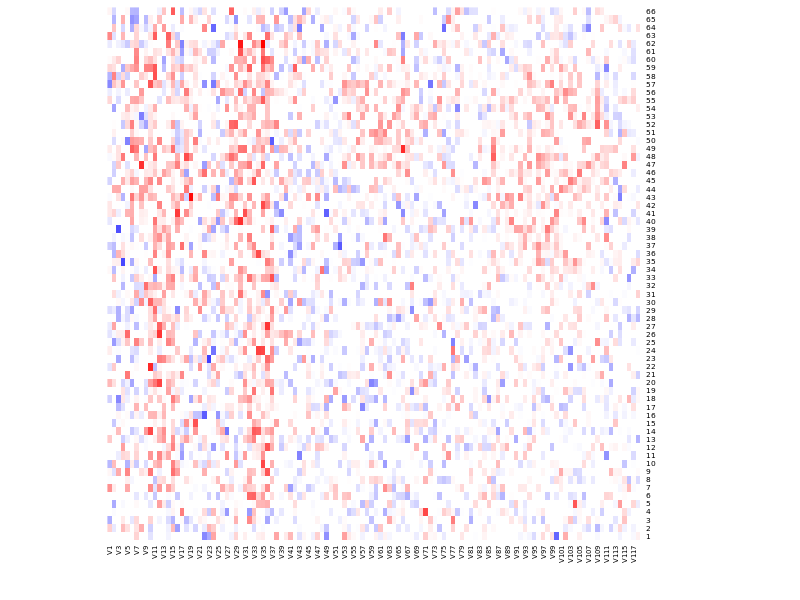
\includegraphics[width=\textwidth]{images/heatmap_logistique_simple_simu_medium_easy.png}}
        \end{minipage}
        \begin{minipage}{0.30\textwidth}
            \centering
            \subfloat[tensor $R: 10$ $(\sigma_{\bm{\beta}}, \sigma_{\text{noise}}) = (0.1,0.8) $\label{fig:easy_multiway}]{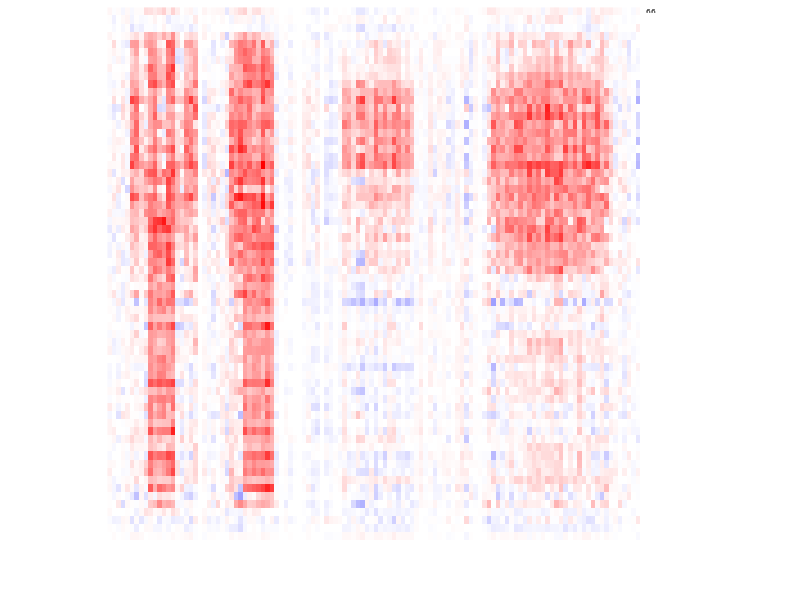
\includegraphics[width=\textwidth]{images/heatmap_logistic_multibloc_simu_4000_medium_easy_multiway.png}}
        \end{minipage}
        \begin{minipage}{0.30\textwidth}
            \centering
            \subfloat[T.M. $R: (6,1,1)$ $(\sigma_{\bm{\beta}}, \sigma_{\text{noise}}) = (0.1,0.8) $\label{fig:easy_multiblock}]{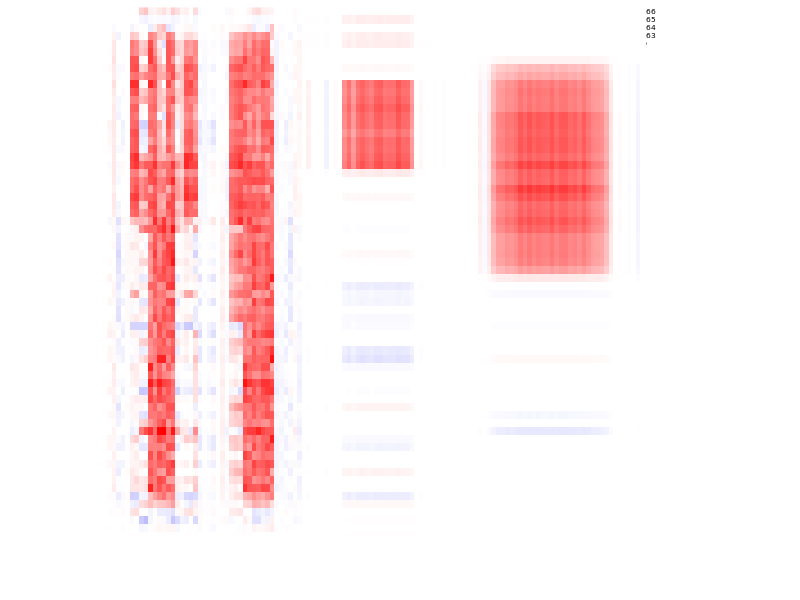
\includegraphics[width=\textwidth]{images/heatmap_logistic_multibloc_simu_4000_medium_easy.png}}
        \end{minipage}
    \end{figure}
\end{frame}

\begin{frame}
    \section{liver tumor data}
    \subsection{with pyradiomics}
\end{frame}

\begin{frame}
    \frametitle{Features extraction with pyradiomics \cite{pyradio}}
    Extraction of $\simeq  100$ features (about intensities, shape, texture) for each $2$D or $3$D image.\\[10 pt]
    \begin{figure}
        \centering
        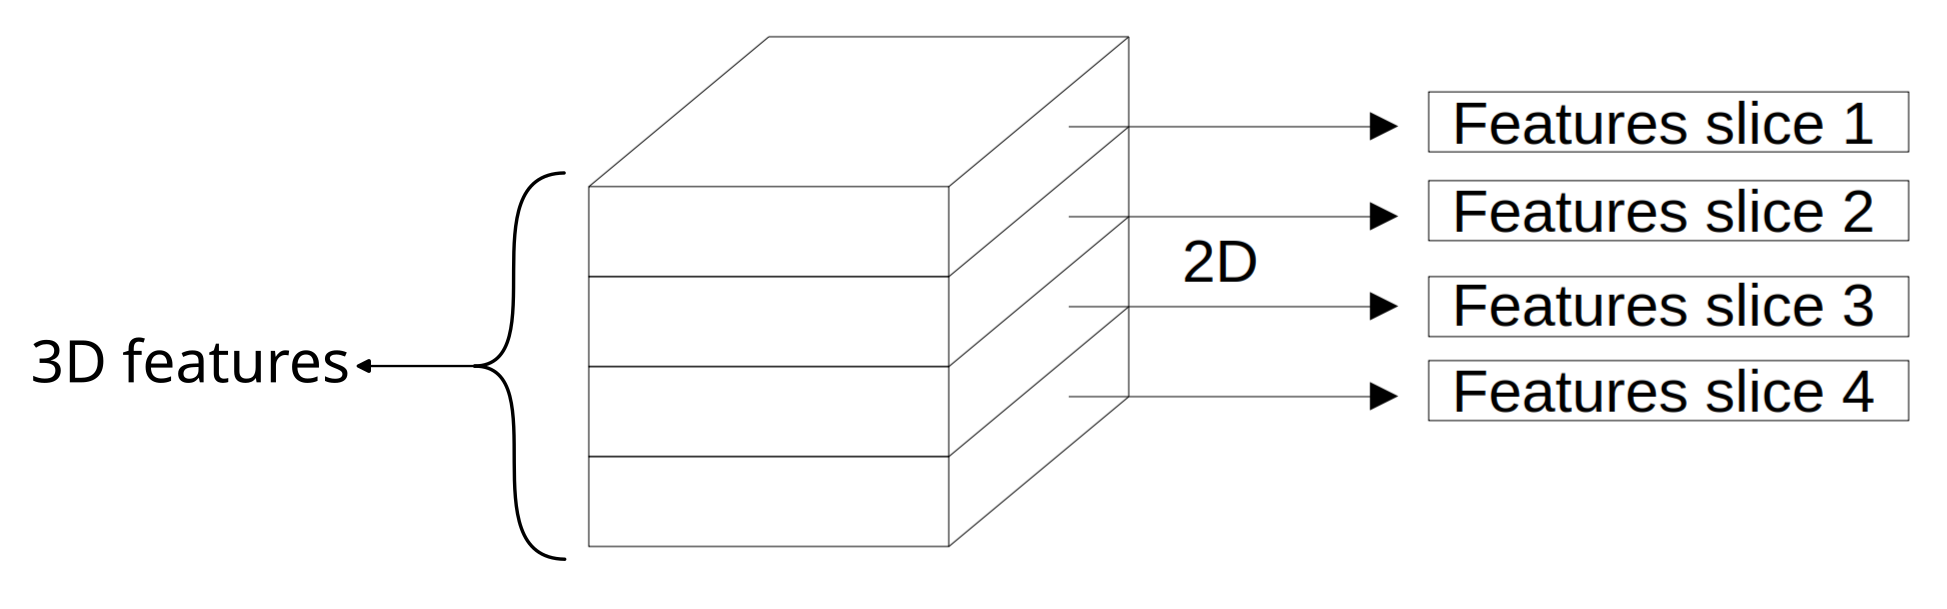
\includegraphics[scale = 0.15]{images/features.png}
        \caption{Features extraction with pyradiomics of an RMI image composed of $4$ slices}
    \end{figure}
\end{frame}

\begin{frame}
    \frametitle{Features extraction in 3D}
    Each radio $\rightarrow$ 1 particular spacing along $(x,y,z)$\\[10 pt]
    \textbf{But} : Calculations of pyradiomics only use voxels (= 3D pixels).\\[10 pt]
    Not always meaningful if the scale changes at each radio (e.g. for Gray Level Run Length Matrix, based on number allignments of pixels of same intensity)\\[10 pt]
    \textbf{Solution}: Standardize the spacing along $(x,y,z)$. Allowed by resampling (interpolation) of the image.
\end{frame}

\begin{frame}
    \frametitle{Features extraction in 2D}
    \vspace{5 pt}
    Slices along z axis $\rightarrow$ same spacing along $(x,y)$\\[5 pt]
    \textbf{Difficulty} Tumors are of variable locations sizes and shapes in the frontal plane (front - back plane)
    \begin{figure}
        \begin{minipage}{0.45\textwidth}
            \centering
            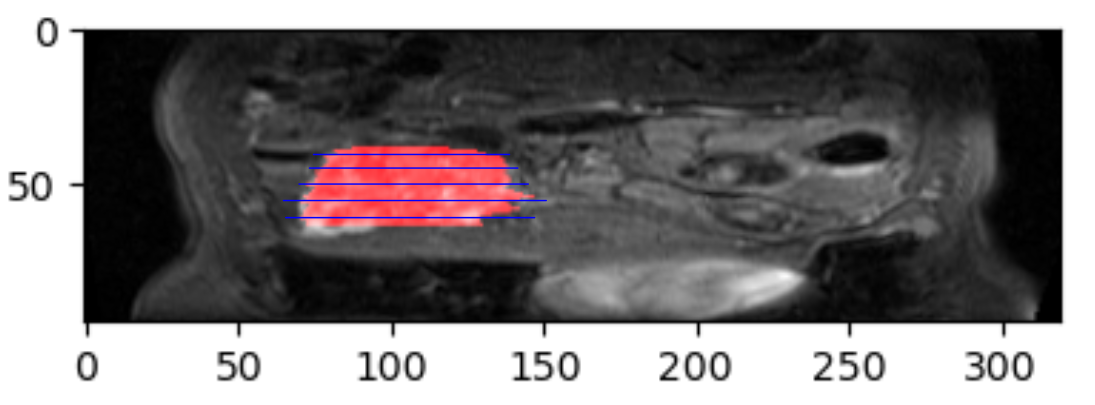
\includegraphics[scale = 0.125]{images/slices_big.png}
            \caption{Extracting 5 slices in a big tumor}
        \end{minipage}
        \hspace{0.03\textwidth} 
        \begin{minipage}{0.45\textwidth}
            \centering
            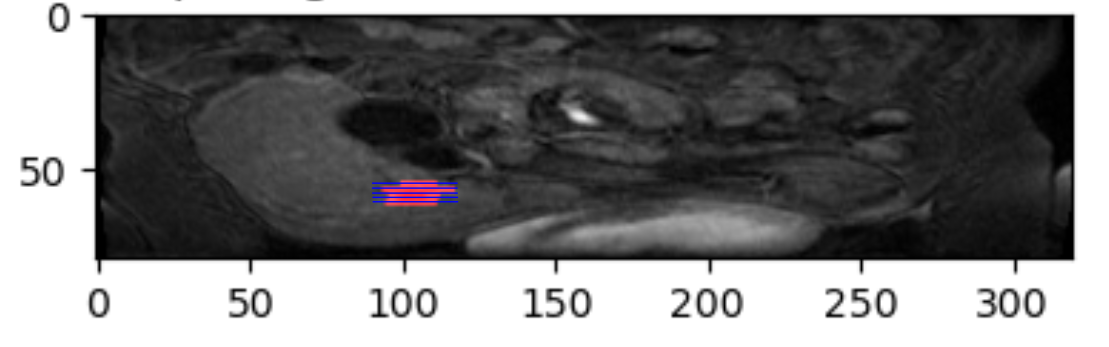
\includegraphics[scale = 0.18]{images/slices_small.png}
            \caption{Extracting 5 slices in a small tumor}
        \end{minipage}
    \end{figure}
\end{frame}

\begin{frame}
    \frametitle{Features extraction in 2D}
    Every slice not equally informative:
    \begin{figure}
        \centering
        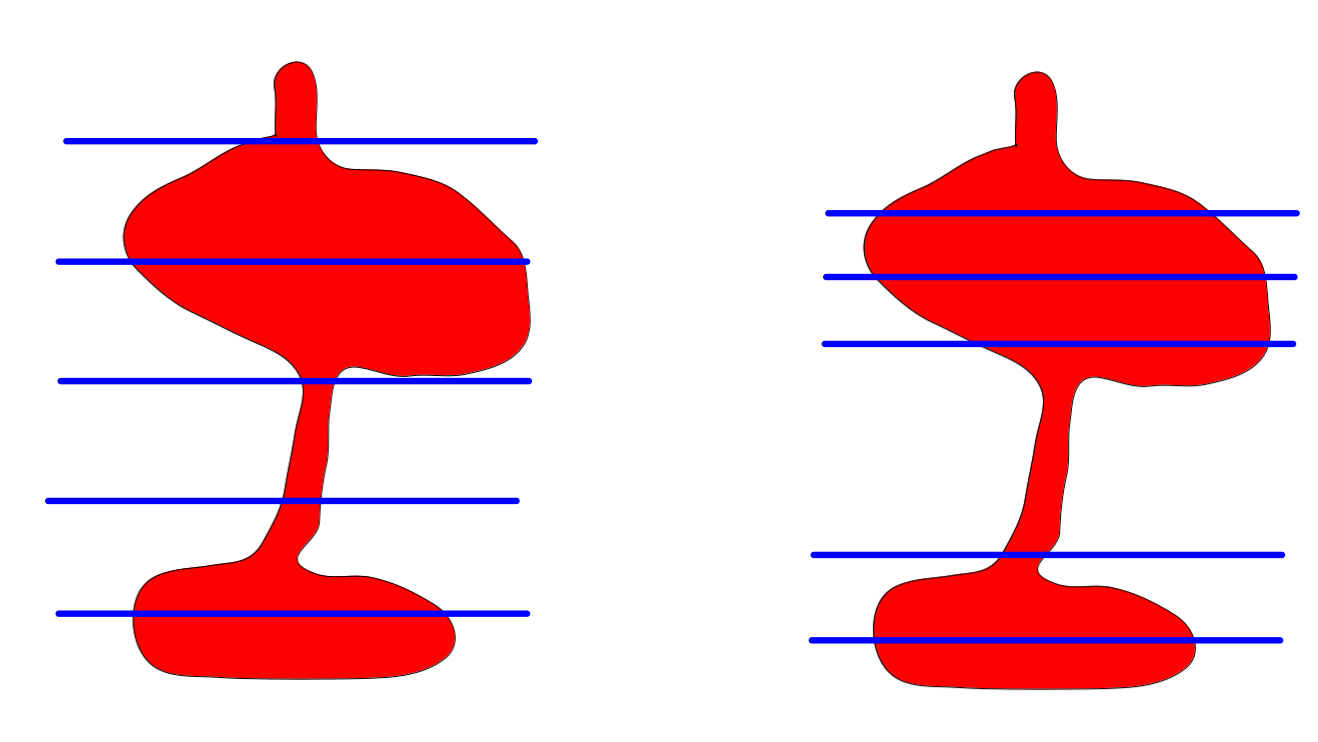
\includegraphics[scale = 0.2]{images/bad_shape.png}
        \caption{Slicing relative to the depth vs. relative to the volume travelled in the tumor}
    \end{figure}
\end{frame}

% \begin{frame}
%     \frametitle{Features extraction in 2D}
%     \textbf{Solution}: Selecting $5$ slices equally spaced along the cumulated volume axis
%     \begin{figure}
%         \centering
%         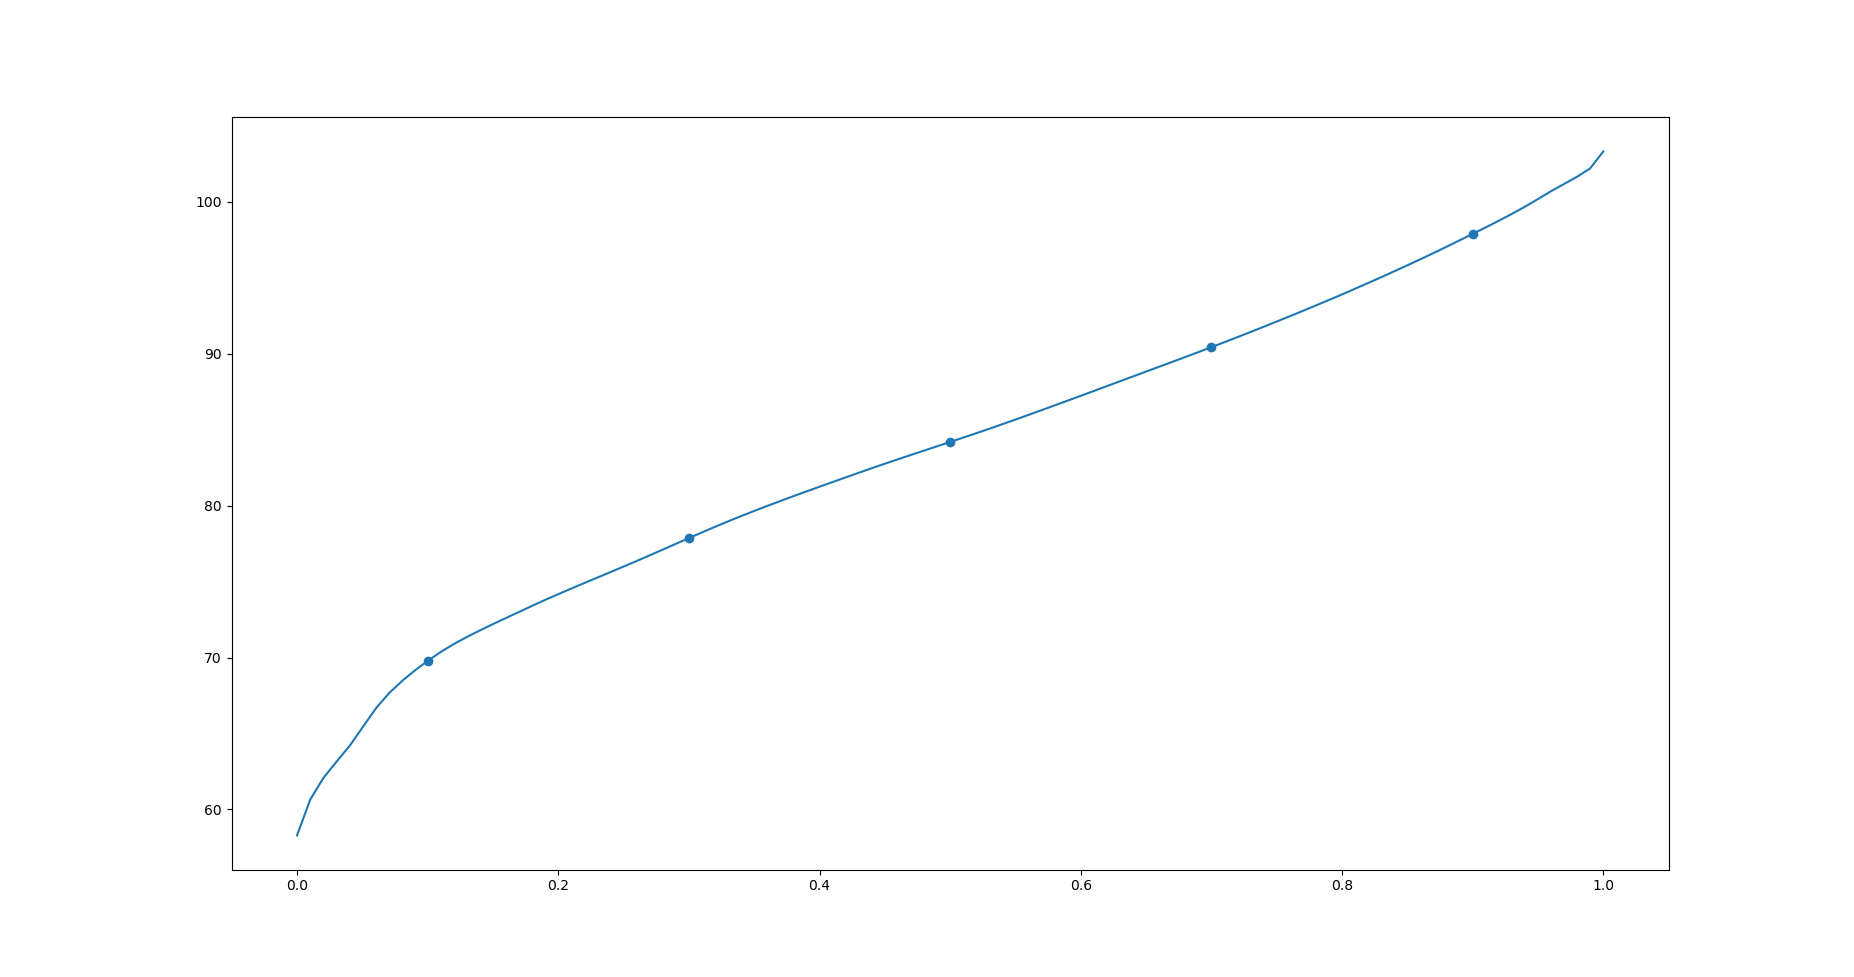
\includegraphics[scale = 0.15]{images/curve_points.png}
%         \caption{Curve of the depth travelled in the liver  (in $mm$) as a function of the standardized cumulated volume of the tumor. The points represent the selected slices.}
%     \end{figure}
% \end{frame}

\begin{frame}
    \frametitle{Results}
    \begin{table}[H]
        \centering
        \label{tab:result_real}
        \renewcommand{\arraystretch}{1.2} 
        \begin{adjustbox}{center}
        \begin{tabular}{|>{\centering\arraybackslash}m{1.4cm}|>{\centering\arraybackslash}m{1.1cm}|>{\centering\arraybackslash}m{1.1cm}|>{\centering\arraybackslash}m{1.1cm}|>{\centering\arraybackslash}m{1.1cm}|>{\centering\arraybackslash}m{1.1cm}|>{\centering\arraybackslash}m{1.1cm}|}
            \cline{1-7}
            Type of data & lasso & g.l. (block) & g.l. (time)& g.l. (var) & tensor & tensor blocks\\
            \cline{1-7} 
            3D & $0.74 \pm 0.04$& $0.78 \pm 0.03$ & $0.76 \pm 0.03$ & $0.73 \pm 0.03$ & $0.77 \pm 0.03$ & $0.77 \pm 0.03$ \\
            \cline{1-7}
    
        \end{tabular}
        
    \end{adjustbox}
    \parbox{0.9\textwidth}{
    \vspace{0.2 cm}    
    \centering \small cross validated area under curve (AUC) on 3D real data}
    \vspace{0.3 cm}
    
    \begin{adjustbox}{center}
    \begin{tabular}{|>{\centering\arraybackslash}m{1.2cm}|>{\centering\arraybackslash}m{1cm}|>{\centering\arraybackslash}m{1cm}|>{\centering\arraybackslash}m{1cm}|>{\centering\arraybackslash}m{1cm}|>{\centering\arraybackslash}m{1cm}|>{\centering\arraybackslash}m{1cm}|>{\centering\arraybackslash}m{1cm}|}
        \cline{1-8}
        Type of data & lasso & g.l. (block) & g.l. (slice)& g.l. (time)& g.l. (var) & tensor & tensor blocks\\
        \cline{1-8} 
        2D & $0.73 \pm 0.03$ & $0.71 \pm 0.03$ & $0.70 \pm 0.04$ & $0.71 \pm 0.03 $  & $0.71 \pm 0.03$ & $0.66 \pm 0.04$ & $0.71 \pm 0.03$ \\
        \cline{1-8}
    \end{tabular}
    \end{adjustbox}
    \parbox{0.9\textwidth}{
    \vspace{0.2 cm}    
    \centering \small Cross validated area under curve (AUC) on 2D real data}
    \end{table}
\end{frame}

\subsection{latest data}

\begin{frame}
    \frametitle{Latest data}
    12 binary features determined by radiologists (late enhancement, non peripheral washout etc...) + sex and existence of chronical disease\\[10 pt]
    With lasso model:
    \begin{itemize}
        \item AUC: $0.97 \pm 0.02$\\[10 pt]
        \item balanced accuracy: $0.88 \pm 0.05$
        \end{itemize}
    Would be interesting to test other models...
\end{frame}

\begin{frame}
    \frametitle{features importance}
    \begin{figure}
        \centering
        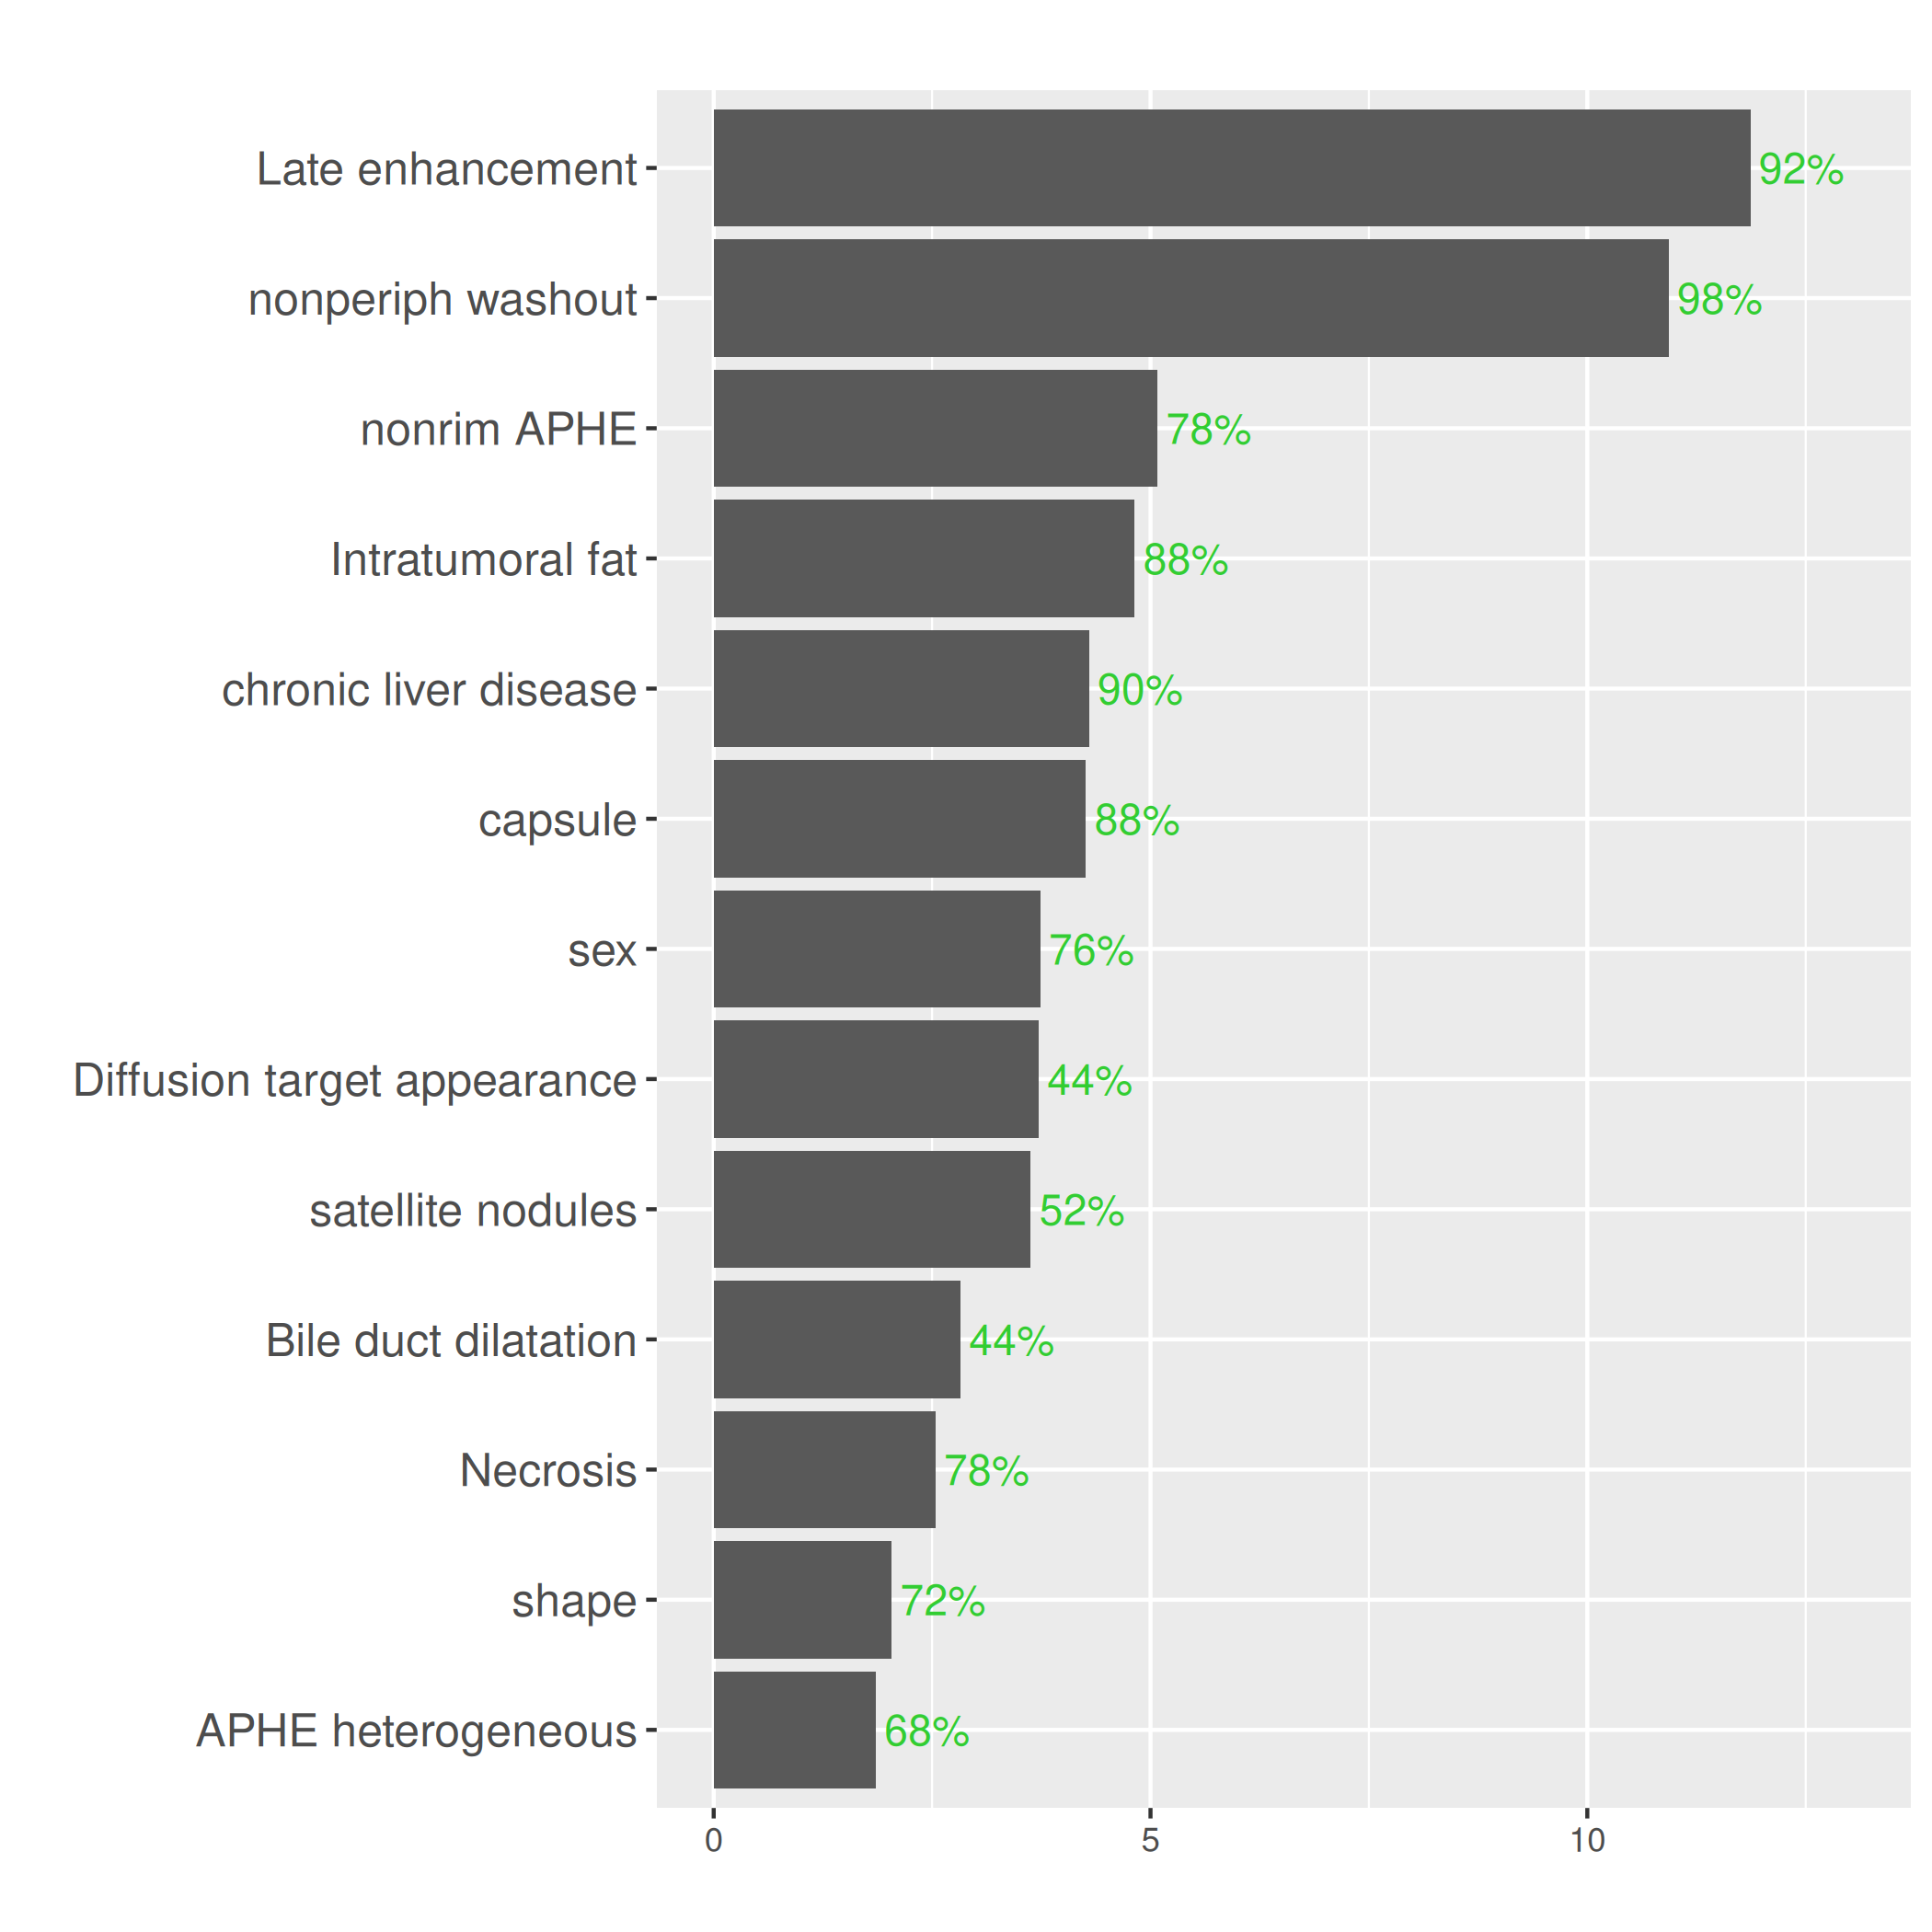
\includegraphics[scale = 0.38]{images/barplot_final.png}
        \caption{Features importance with lasso (in green percentage of runs with non null coefficient)}
    \end{figure}
\end{frame}

\begin{frame}
    \frametitle{Possible extensions}
    Testing other penalizations (group lasso, elastic net)\\[10 pt]
    Extending the multiblock approach to other classical machine learning algorithms (other GLMs, SVM etc...). Comparing it to CNN.\\[10 pt]
    Testing other models on the latest data (in order to obtain a model that can be deployed in the hospital).\\[10 pt]
    Implementing the multiblock code in C for increased speed (currently quite slowin R)
\end{frame}

\begin{frame}
    \section{Retrospective Analysis}
\end{frame}

\begin{frame}
    \frametitle{Impact of the internship on me}
    Direct impact: continuing in thesis (increase in motivation for research activities)\\[10 pt]
    Soft skills in machine learning: become more critical vs results, searching for other data whenever possible\\[10 pt]
    Being part of a team in a scientific context (not only 1 supervisor): importance of communication and reporting (even when no writen documents)\\[10 pt]
    The reasearch in machine learning: an accessible world
\end{frame}


\begin{frame}
    \frametitle{Consequences of the internship}
    A promising framework for the diagnosis of liver tumors\\[10 pt]
    The simulation part of an article on the multiblock tensor 
    More information about the correct context for using that kind of models\\[10 pt]
    An ethically positive impact (controllable deployment, a precise need, no replacement of humans...)
    
\end{frame}

\begin{frame}
    \frametitle{Conclusion}
    A good representation of a research work (and its challenges)\\[10 pt]
    Supportive, available and Calm supervision (even as deadlines approach)\\[10 pt]
    Looking forward to continuing in this direction
\end{frame}

\begin{frame}
\section*{bibliography}
\end{frame}


\begin{frame}[allowframebreaks] 
    \bibliographystyle{plain}
    \bibliography{bibliography.bib} 
    \end{frame}



\end{document}